\documentclass[12pt,a4paper]{article}
\usepackage[top=2cm,bottom=2cm,left=2cm,right=2cm]{geometry} %marg
\usepackage{polski}                                          %pl
\usepackage[cp1250]{inputenc}
\usepackage[OT4]{fontenc}                                    %font
\usepackage{graphicx}                                  %dodanie grafiki
\usepackage{enumerate}                                % a)b)c)....

\newtheorem{zad}{Zadanie}[section]

\title{Funkcje Trygonometryczne}
\author{Kevin Sarfo}



\begin{document}
\maketitle

\tableofcontents
\newpage
\section{Leckcja}

\subsection{Krótki wstęp}

Funkcje trygonometryczne – funkcje matematyczne wyrażające między innymi stosunki między długościami boków trójkąta prostokątnego względem miar jego kątów wewnętrznych, będące przedmiotem badań trygonometrii.

Funkcje trygonometryczne, choć wywodzą się z pojęć geometrycznych, są rozpatrywane także w oderwaniu od geometrii. W analizie matematycznej są one definiowane m.in. za pomocą szeregów potęgowych lub jako rozwiązania pewnych równań różniczkowych.

Do funkcji trygonometrycznych współcześnie zalicza się: sinus, cosinus (inna pisownia: kosinus), tangens, cotangens (kotangens), secans (sekans), cosecans (kosekans), z czego dwóch ostatnich obecnie rzadko się używa.\cite{od}

Pomimo trudnego opisu nie ma się czego obawiać. Funkcje trygonometryczne nie wymagają wykonywania bardzo skomplikowanych obliczeń takich jak rownanie (\ref{delta})

\begin{equation}
\begin{array}{c} 
\label{delta}
a_l& =&\sqrt{\frac{(6,14-6,15)^2+(6,18-6,15)^2+(6,12-6,15)^2+
(6,15-6,15)^2+(6,16-6,15)^2}{4}} \\
=0,022360679=0,023
\end{array}
\end{equation}






\subsection{Proste Wyjaśnienie}

Narysujmy dowolny trójkąt prostokątny i oznaczmy jeden z jego kątów ostrych literką α.

%%%%%% miejsce na obrazek
\begin{figure}
\centering
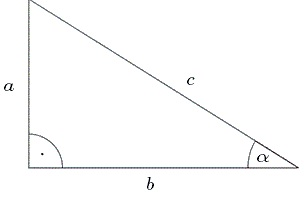
\includegraphics[width=5cm]{troj}
\caption{Trójkąt prostokątny z oznaczeniami}
\label{fig:obrazek troj}
\end{figure}


Literkami a oraz b oznaczyliśmy przyprostokątne trójkąta prostokątnego.
Literką c oznaczyliśmy przeciwprostokątną trójkąta prostokątnego.
Teraz możemy podać definicje funkcji trygonometrycznych (1-sinus, 2-cosinus, 3-tangens, 4-cotangens):

\begin{center}
\label{row}
1) $sinα=\frac{a}{c}$,
\label{row}
2) $cosα=\frac{b}{c}$,
\label{row}
3) $tgα=\frac{a}{b}$,
\label{row}
4) $ctgα=\frac{b}{a}$.

\end{center}

\cite{od1}

\begin{figure}
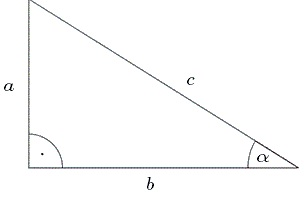
\includegraphics[width=3cm, angle=25]{troj}
\end{figure}


\newpage
\section{Zadania}

\subsection{Proste zadania}

\begin{zad}
Oblicz pozostałe wartości funkcji trygonometrycznych trójkąta prostokątnego:

\begin{enumerate}[a)]
\item $a=4 , sinα=\frac{4}{5}$ Skorzystaj z \ref{row}
\item $b=6 cosα=\frac{1}{2}$   Skorzystaj z \ref{row}
\item $a=8 ,tgα=1$             Skorzystaj z \ref{row}  
\item $b=5 ctgα=\frac{7}{10}$  Skorzystaj z \ref{row}
\end{enumerate}

\end{zad}

\begin{zad}
Oblicz wartość wyrażenia: sin 45° · tg 60° · cos230°.
\end{zad}

\begin{zad}
Drabina o długości 3m jest oparta o mur pod kątem  do poziomu. Na jaką wysokość sięga drabina?
\end{zad}

\begin{zad}
Samolot wystartował pod kątem. Jaką drogę w powietrzu pokonał w momencie, gdy znalazł się na wysokości 200m?
\end{zad}

\begin{zad}
Kąt ostry trapezu równoramiennego ma miarę. Oblicz jego pole, jeżeli jego podstawy mają długość 12cm i 6cm.
\end{zad}

\subsection{Bardziej zaawansowane zadania}


\begin{zad}
Zbadaj, czy istnieje kąt ostry dla którego $tgα=\frac{3}{4}$ i $sinα=\frac{3}{5}$
\end{zad}
α i β
\begin{zad}
W trójkącie prostokątnym o kątach α i β (α < β) dane są długości przyprostokątnych 4 i 6. Oblicz wartość wyrażenia $tg^{2}α-3sinα·\frac{1}{cosβ}$
\end{zad}

\section{Tabela funkcji trygonomentrycznych}

\begin{tabular}{|c|c|c|c|} \hline
α & 30° & 45° & 60° \\
sinα & $\frac{1}{2}$ & $\farc{\sqrt{2}}{2}$ &   $\farc{\sqrt{3}}{2}$ \\
cosα & $\farc{\sqrt{3}}{2}$ & $\farc{\sqrt{2}}{2}$ & $\frac{1}{2}$\\
tgα &   $\farc{\sqrt{3}}{3}$& 1  &  $\sqrt{3}$\\
ctgα & $\sqrt{3}$ & 1 & $\farc{\sqrt{3}}{3}$\\
\hline \hline
\end{tabular}


\section{Zakończenie}
Teraz już wiesz że trygonometria nie jest tak cięzka jak równanie (\ref{delta})

\begin{figure}

\includegraphics[width=3cm, angle=25]{einstein}
\end{figure}

\begin{figure}
\centering

\includegraphics[width=5cm]{einstein}
\caption{Karykatura Alberta Einstein'a}
\label{fig:obrazek troj}
\end{figure}

\center Mam nadzieję że załączony materiał pomoże wielu licealistą w nauce.
\center :)


\newpage

\section{Bibliografia}

\begin{thebibliography}{9}
\bibitem{od}Wojciech Babiański: \emph{Matematyka - Zakres rozszerzony}
\bibitem{od1}Karpiński Marcin : \emph{Matematyka 1. Podręcznik dla liceum}

\end{thebibliography}

\end{document}
